% $Header: /home/vedranm/bitbucket/beamer/solutions/generic-talks/generic-ornate-15min-45min.en.tex,v 90e850259b8b 2007/0\frac{1}{2}8 20:48:30 tantau $
\documentclass{beamer}
%\documentclass[handout]{beamer}
\usefonttheme[onlymath]{serif}
% This file is a solution template for:
\usepackage{algorithm}
\usepackage{algpseudocode}
\usepackage{tikz}

\usepackage{animate}
% - Giving a talk on some subject.
% - The talk is between 15min and 45min long.
% - Style is ornate.
% Copyright 2004 by Till Tantau <tantau@users.sourceforge.net>.
%
% In principle, this file can be redistributed and/or modified under
% the terms of the GNU Public License, version 2.
%
% However, this file is supposed to be a template to be modified
% for your own needs. For this reason, if you use this file as a
% template and not specifically distribute it as part of a another
% package/program, I grant the extra permission to freely copy and
% modify this file as you see fit and even to delete this copyright
% notice. 

\mode<presentation>
{
  \usetheme{Warsaw}
  % or ...

  \setbeamercovered{transparent}
  % or whatever (possibly just delete it)
}
\setbeamertemplate{navigation symbols}{} 

\usepackage[english]{babel}
% or whatever

\usepackage[latin1]{inputenc}
% or whatever
\useoutertheme{default}

\usepackage{times}
\usepackage[T1]{fontenc}
% Or whatever. Note that the encoding and the font should match. If T1
% does not look nice, try deleting the line with the fontenc.
\newcommand{\beforeverb}{\footnotesize}
\newcommand{\afterverb}{\normalsize}

\title[Fast Fourier Transformation] % (optional, use only with long paper titles)
{Lecture 14}

\subtitle
{Fast Fourier Transformation} % (optional)

\author[Ying-Jer Kao] % (optional, use only with lots of authors)
{Ying-Jer Kao}
% - Use the \inst{?} command only if the authors have different
%   affiliation.

\institute[National Taiwan University] % (optional, but mostly needed)
{
  Department of Physics\\
 National Taiwan University
  }
% - Use the \inst command only if there are several affiliations.
% - Keep it simple, no one is interested in your street address.

\date[Numerical Analysis and Programming] % (optional)
{\today}

\subject{Talks}
% This is only inserted into the PDF information catalog. Can be left
% out. 



% If you have a file called "university-logo-filename.xxx", where xxx
% is a graphic format that can be processed by latex or pdflatex,
% resp., then you can add a logo as follows:

% \pgfdeclareimage[height=0.5cm]{university-logo}{university-logo-filename}
% \logo{\pgfuseimage{university-logo}}



% Delete this, if you do not want the table of contents to pop up at
% the beginning of each subsection:
%\AtBeginSubsection[]
%{
%  \begin{frame}<beamer>{Outline}
%    \tableofcontents[currentsection,currentsubsection]
%  \end{frame}
%}


% If you wish to uncover everything in a step-wise fashion, uncomment
% the following command: 

%\beamerdefaultoverlayspecification{<+->}


\begin{document}

\begin{frame}
  \titlepage
\end{frame}

\begin{frame}{Outline}
  \tableofcontents
  % You might wish to add the option [pausesections]
\end{frame}


% Since this a solution template for a generic talk, very little can
% be said about how it should be structured. However, the talk length
% of between 15min and 45min and the theme suggest that you stick to
% the following rules:  

% - Exactly two or three sections (other than the summary).
% - At *most* three subsections per section.
% - Talk about 30s to 2min per frame. So there should be between about
%   15 and 30 frames, all told.
\section[Introduction]{Introduction}
\begin{frame}{Introduction}
\begin{itemize}
    \item Discrete Fourier Transformation (DFT) is a powerful tool in signal processing.
    \item The DFT of a sequence of length $N$ requires $O(N^2)$ operations.
    \item The Fast Fourier Transformation (FFT) is an algorithm that reduces the number of operations to $O(N\log N)$.
    \item The FFT is a divide-and-conquer algorithm that recursively divides the DFT into smaller DFTs.
    \item The FFT is widely used in many applications, such as signal processing, image processing, and data compression.
    
\end{itemize}
\end{frame}
\section{Discrete Fourier Transformation}

\begin{frame}{Discrete Fourier Transformation}
    \begin{itemize}
        \item The DFT of a sequence $x_0,x_1,\ldots,x_{N-1}$ is defined as
        \[
        X_k = \sum_{n=0}^{N-1}x_n e^{-2\pi i k n/N},\quad k=0,1,\ldots,N-1.
        \]
        \item The inverse DFT is defined as
        \[
        x_n = \frac{1}{N}\sum_{k=0}^{N-1}X_k e^{2\pi i k n/N},\quad n=0,1,\ldots,N-1.
        \]
        \item The DFT of a sequence of length $N$ requires $O(N^2)$ operations.
    \end{itemize}
\end{frame}
\begin{frame}{Discrete Fourier Transformation}
    \begin{itemize}
        \item The DFT can be computed using the matrix-vector multiplication
        \[
        X = W_N x,
        \]
        where $W_N$ is the $N\times N$ matrix defined as
        \[
        W_N = \begin{bmatrix}
        1 & 1 & 1 & \cdots & 1\\
        1 & w & w^2 & \cdots & w^{N-1}\\
        1 & w^2 & w^4 & \cdots & w^{2(N-1)}\\
        \vdots & \vdots & \vdots & \ddots & \vdots\\
        1 & w^{N-1} & w^{2(N-1)} & \cdots & w^{(N-1)(N-1)}
        \end{bmatrix},
        \]
        and $w = e^{-2\pi i/N}$.
    \end{itemize}
\end{frame}
\section{Fast Fourier Transformation}
\begin{frame}{Fast Fourier Transformation}
    \begin{itemize}
     \item Using a divde-and-conquer approach, the DFT can be computed in $O(N\log N)$ operations.
     \item The DFT of a sequence of length $N=2^m$ can be computed by computing the DFTs of the even-indexed and odd-indexed elements of the sequence.
     \item The DFT of the even-indexed elements is the \textbf{sum} of the DFTs of the even-indexed and odd-indexed elements of the original sequence.
     \item The DFT of the odd-indexed elements is the \textbf{difference} of the DFTs of the even-indexed and odd-indexed elements of the original sequence.
     \item The FFT algorithm recursively divides the DFT into smaller DFTs until the length of the sequence is 1.
    \end{itemize}

\end{frame}
\begin{frame}{FFT: Cooley-Tukey Alogirhtm}
    \begin{itemize}
        \item Consider a sequence of length $N=2^m$.
        \item Let $x_0,x_1,\ldots,x_{N-1}$ be the sequence.
        \item The DFT of the sequence can be computed as follows:
        \beforeverb
        \[
            X_k=\sum_{m=0}^{N / 2-1} x_{2 m} e^{-\frac{2 \pi i}{N}(2 m) k}+\sum_{m=0}^{N / 2-1} x_{2 m+1} e^{-\frac{2 \pi i}{N}(2 m+1) k}
        \]
        \afterverb
        \item Factor out the common factor $e^{-\frac{2 \pi i}{N} k}$ in the second term, we have
        \beforeverb
        \begin{align*}
            X_k&=\underbrace{\sum_{m=0}^{N / 2-1} x_{2 m} e^{-\frac{2 \pi i}{N / 2} m k}}_{\text {DFT of even-indexed part of } x_n}+e^{-\frac{2 \pi i}{N} k} \underbrace{\sum_{m=0}^{N / 2-1} x_{2 m+1} e^{-\frac{2 \pi i}{N / 2} m k}}_{\text {DFT of odd-indexed part of } x_n}\\
            &=E_k+e^{-\frac{2 \pi i}{N} k} O_k \quad \text { for } k=0, \ldots, \frac{N}{2}-1 .
        \end{align*}
        \afterverb
        Note the equality applies to all $k$s but $E_k$ and $O_k$ are computed for $k=0,1,\ldots,N/2-1$.
    \end{itemize}
\end{frame}
\begin{frame}
\begin{itemize}
    \item We also have 
    \beforeverb 
        \begin{align*}
            X_{k+\frac{N}{2}} & =\sum_{m=0}^{N / 2-1} x_{2 m} e^{-\frac{2 \pi i}{N / 2} m\left(k+\frac{N}{2}\right)}+e^{-\frac{2 \pi i}{N}\left(k+\frac{N}{2}\right)} \sum_{m=0}^{N / 2-1} x_{2 m+1} e^{-\frac{2 \pi i}{N / 2} m\left(k+\frac{N}{2}\right)} \\
            & =\sum_{m=0}^{N / 2-1} x_{2 m} e^{-\frac{2 \pi i}{N / 2} m k} e^{-2 \pi m i}+e^{-\frac{2 \pi i}{N} k} e^{-\pi i} \sum_{m=0}^{N / 2-1} x_{2 m+1} e^{-\frac{2 \pi i}{N / 2} m k} e^{-2 \pi m i} \\
            & =\sum_{m=0}^{N / 2-1} x_{2 m} e^{-\frac{2 \pi i}{N / 2} m k}-e^{-\frac{2 \pi i}{N} k} \sum_{m=0}^{N / 2-1} x_{2 m+1} e^{-\frac{2 \pi i}{N / 2} m k} \\
            & =E_k-e^{-\frac{2 \pi i}{N} k} O_k
        \end{align*}
    \afterverb
   
    \item Therefore, the DFT of length $N$ can be recursively expressed in terms of two DFTs of size $N/2$,
    \begin{align*}
        X_k & =E_k+e^{-\frac{2 \pi i}{N} k} O_k \\
        X_{k+\frac{N}{2}} & =E_k-e^{-\frac{2 \pi i}{N} k} O_k
        \end{align*}
    \item Recursively compute the DFTs of the even-indexed and odd-indexed elements of the sequence until the length of the sequence is 1.
\end{itemize}
\end{frame}
\begin{frame}
\centerline{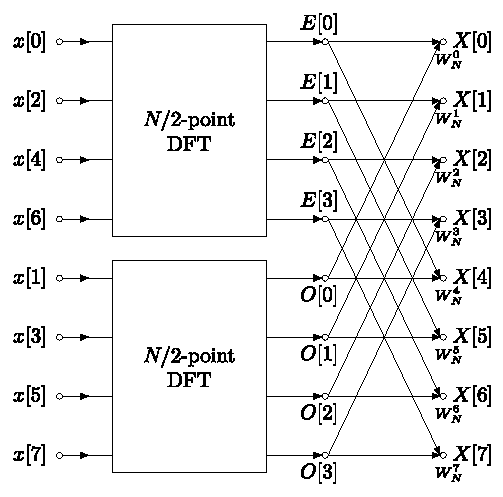
\includegraphics[width=0.8\textwidth]{DIT-FFT-butterfly.pdf}}
\end{frame}

\begin{frame}{FFT: PseudoCode}
\beforeverb
\begin{algorithmic}
\Procedure{FFT}{$x$}
    \State $N \gets \text{length}(x)$
    \If{$N == 1$}
        \State \Return $x$
    \EndIf
    \State $w_N \gets e^{-2\pi i / N}$
    \State $x_{\text{even}} \gets x[0::2]$
    \State $x_{\text{odd}} \gets x[1::2]$
    \State $X_{\text{even}} \gets \text{FFT}(x_{\text{even}})$
    \State $X_{\text{odd}} \gets \text{FFT}(x_{\text{odd}})$
    \State $X \gets \text{array of zeros of length } N$
    \For{$k = 0$ to $N/2 - 1$}
        \State $X[k] \gets X_{\text{even}}[k] + w_N^k \cdot X_{\text{odd}}[k]$
        \State $X[k + N/2] \gets X_{\text{even}}[k] - w_N^k \cdot X_{\text{odd}}[k]$
    \EndFor
    \State \Return $X$
\EndProcedure
\end{algorithmic}
\afterverb
\end{frame}
\end{document}


